\documentclass[UTF8,a4paper]{ctexart}
\usepackage[utf8]{inputenc}
\usepackage{amsmath}
\usepackage{pdfpages}
\usepackage{graphicx}
\usepackage{wrapfig}
\usepackage{listings}
\usepackage{hyperref}
\usepackage{multicol}
\title{单管放大电路的系统辨识和控制器设计}
\author{张蔚桐\ 2015011493\ 自55}
\begin {document}
\newcommand{\tabincell}[2]{\begin{tabular}{@{}#1@{}}#2\end{tabular}}
\maketitle
\tableofcontents
\clearpage
\section{引言}
在模拟电子技术课程中,对于放大电路的高频特性,我们通过对晶体管的工作原理分析,引入了混合$\pi$电路,完成了对电路频率特性的研究。然而实际应用过程中,这种方法往往存在某些问题,下面分点简述如下。
\begin{enumerate}
\item 电路计算模型复杂

回顾三极管的混合$\pi$及其简化模型,可以看出其电路模型尽管经过很大程度的简化,电路的模型仍然十分复杂。因此,如果将混合$\pi$模型推广到复合管电路或者多级运放甚至更大规模的集成电路中,必然出现计算量过大的情况。
因此,在工程中,不论采用仿真计算或手工计算,均要耗费相当大的工程量。
\item 模型存在误差

不论是晶体管的中频段等效模型还是混合$\pi$模型,不可否认的一点是这些模型均存在这一定程度的误差。同时,随着电路的集成和封装,过程中引入的分布电容,接触电阻和其他不可预计的效应是很多的,在更复杂的电路中,这些干扰将进一步的相互耦合,使得简单的简化模型对电路性能的预计变得更加不准确。同时也增大了采用模型刻画电路的难度
\item 全频段分析中的矛盾

在采用混合$\pi$等等效模型对频率响应进行分析时,如果选用了全频段模型,我们势必面对规模较大的电路,虽然能够解出适合于全频段的传递函数,但是在实际工程应用中,我们涉及到的频率往往仅仅是全频段中的一部分。如果采用高/中/低频等效电路,则经常需要考虑简化的模型是否会影响到电路的整体性能描述。什么样的电路元件可以省略,什么样的电路元件不能省略,往往是一个很模糊的概念。高/中/低频等效电路的使用范围也不是一个确切的值,因此在频段分析中存在着过度简化和过度复杂之间界限不清楚的问题
\end{enumerate}

为了解决以上问题,我们回顾控制理论中一个完全相反的思路:通过实验测得的频率特性去完成对传递函数的估计,并进一步设计传递函数的实现。这种基于实验的方法,能够从根本上解决已有模型不能充分描述电路特性的问题,也能够解决电路在集成和封装过程中存在的电阻电容引入难以计算的问题。同时,对要求频率附近的频率特性进行测量,得到适合要求频率范围使用的传递函数,也可以解决对于各个频段模型划分模糊的问题

\section{可行性分析}
我们知道,一个线性系统可以从其bode图等频率响应图中估计出系统的传输函数。对于放大电路而言,由于静态工作点的设置使得静态工作电压远远大于输入的交变电压,因此整个系统完全可以在静态工作点附近进行微偏线性化进行线性模型等效。如图\ref{1},\ref{2}所示,测试电路中采用的输入电压峰峰值为10mV,静态工作点在V的量级。微变电压在静态电压的1\%量级上,采用线性模型进行估计所产生的误差是可以接受的。

\section{实验测量}
在电子技术实验中,在老师的指导下对单管放大电路的频率特性(辐频,相频特性)进行了研究。得到的实验结果如表\ref{tablef1},\ref{tablef2}所示,使用绘图软件绘制其辐频和相频特性曲线如图\ref{bode1}\ref{bode2}所示,其中横坐标采用的是频率的分贝数。从图中我们可以看出这两种静态工作点下的频率特性虽然有所差异,但是基本的模态是相同的,因此下文将就$I_{CQ}=1\rm{mA}$时的情况着重分析,至于$I_{CQ}=2\rm{mA}$时的情况将只给出结论
\begin{figure}
\centering
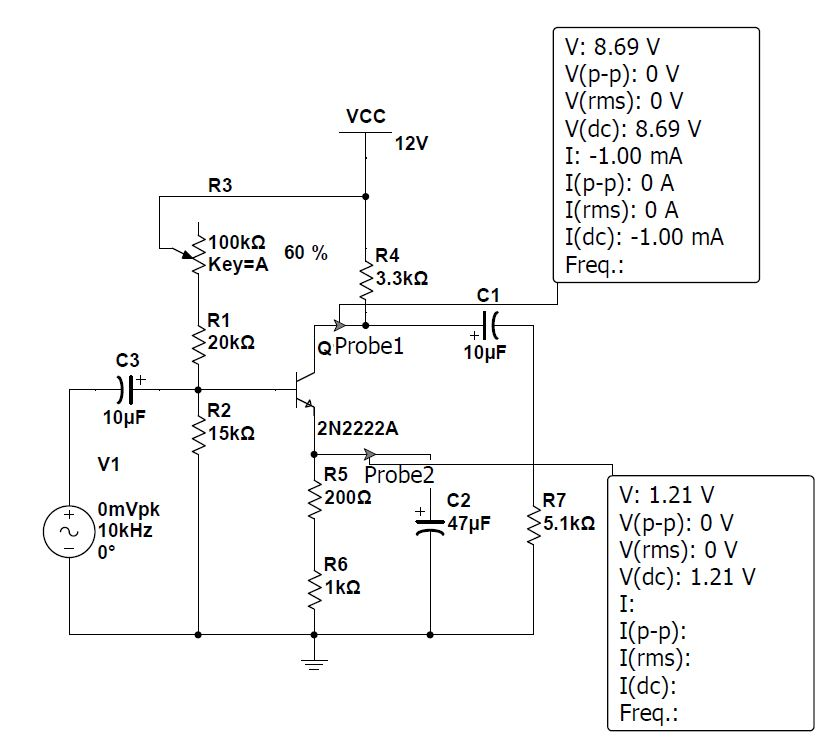
\includegraphics[width=\textwidth]{1.jpg}
\caption{$I_{CQ}=1\rm{mA}$时的电路图}
\label{1}
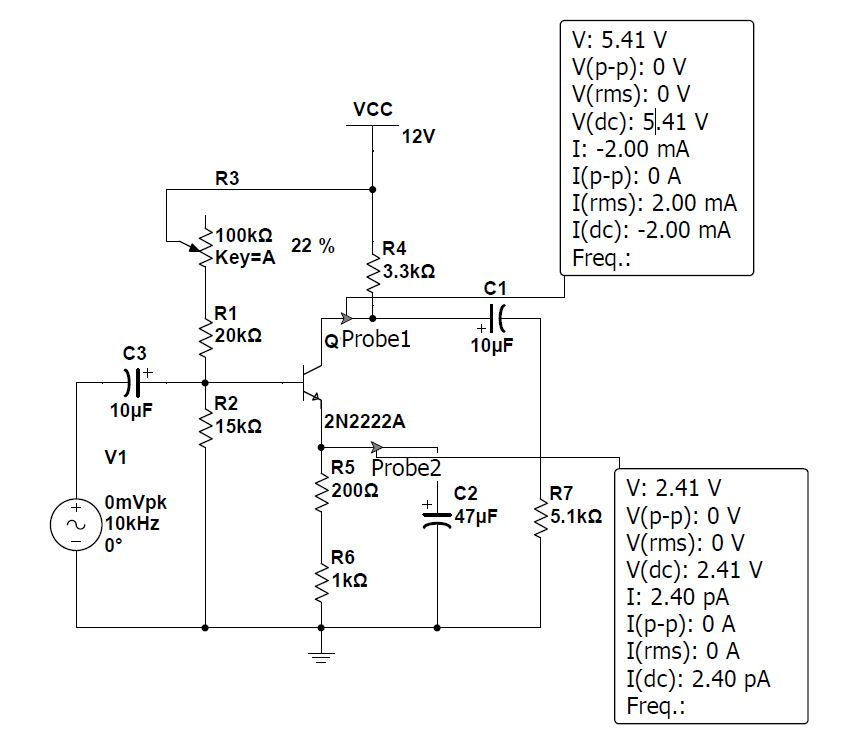
\includegraphics[width=\textwidth]{2.jpg}
\caption{$I_{CQ}=2\rm{mA}$时的电路图}
\label{2}
\end{figure}
\begin{table}
\centering
\begin{multicols}{2}
\caption{$I_{CQ}=1\rm{mA}$时的辐频相频特性}
\label{tablef1}
\begin{tabular}{|c|c|c|}
\hline
\tabincell{c}{$f/\rm{Hz}$}& \tabincell{c}{$|\dot{A}|$} & \tabincell{c}{$\phi$}\\
\hline
$10^{0}$&0.9875&-89.28\\
\hline
$10^{0.5}$&2.1125&-93.8\\
\hline
$10^{1}$&5.2375&-97.2\\
\hline
$10^{1.5}$&14.2875&-111.82\\
\hline
$10^{2}$&32.125&-126.04\\
\hline
$10^{2.5}$&43.875&-157.61\\
\hline
$10^{3}$&47.875&-159.09\\
\hline
$10^{3.5}$&48.25&-166.23\\
\hline
$10^{4}$&48.375&-173.41\\
\hline
$10^{4.5}$&48.125&-180.17\\
\hline
$10^{5}$&45.000&-188.56\\
\hline
$10^{5.5}$&32.250&-223.5\\
\hline
$10^{6}$&12.6625&-270.5\\
\hline
$10^{6.5}$&4.25&---\\
\hline
$10^{7}$&1.325&---\\
\hline
\end{tabular}
\caption{$I_{CQ}=2\rm{mA}$时的辐频相频特性}
\label{tablef2}
\begin{tabular}{|c|c|c|}
\hline
\tabincell{c}{$f/\rm{Hz}$}& \tabincell{c}{$|\dot{A}|$} & \tabincell{c}{$\phi$}\\
\hline
$10^{0}$&0.5025&-59.04\\
\hline
$10^{0.5}$&1.925&-86.52\\
\hline
$10^{1}$&7.650&-94.68\\
\hline
$10^{1.5}$&16.100&-101.0\\
\hline
$10^{2}$&38.000&-124.09\\
\hline
$10^{2.5}$&62.5&-150.71\\
\hline
$10^{3}$&70.5&-167.60\\
\hline
$10^{3.5}$&72.5&-178.02\\
\hline
$10^{4}$&73.00&-183\\
\hline
$10^{4.5}$&72.00&-188.73\\
\hline
$10^{5}$&64.00&-206.03\\
\hline
$10^{5.5}$&36.00&-230.8\\
\hline
$10^{6}$&13.5&-263.2\\
\hline
$10^{6.5}$&4.5&---\\
\hline
$10^{7}$&1.6&---\\
\hline
\end{tabular}
\end{multicols}
\end{table}
\begin{figure}
\centering
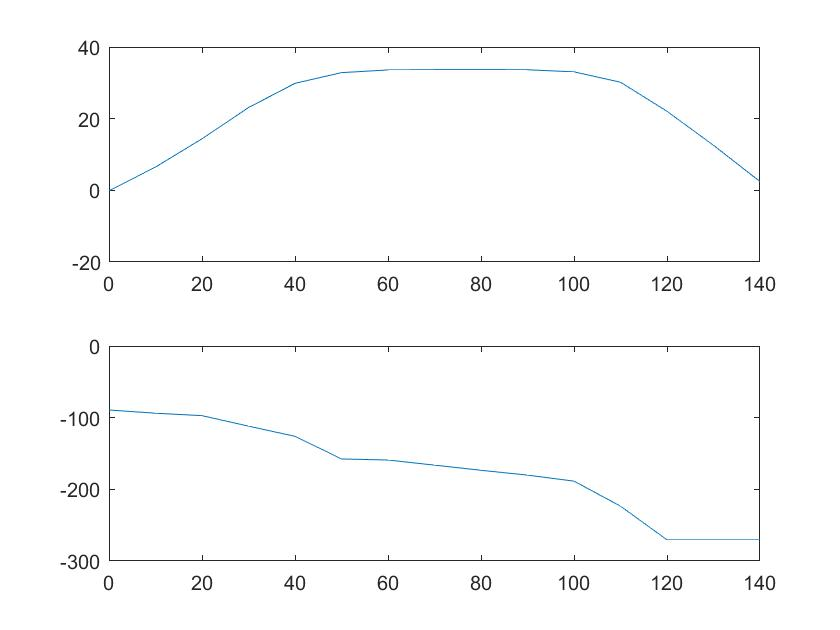
\includegraphics[width=\textwidth]{bode1exp.jpg}
\caption{$I_{CQ}=1\rm{mA}$时的辐频相频特性图}
\label{bode1}
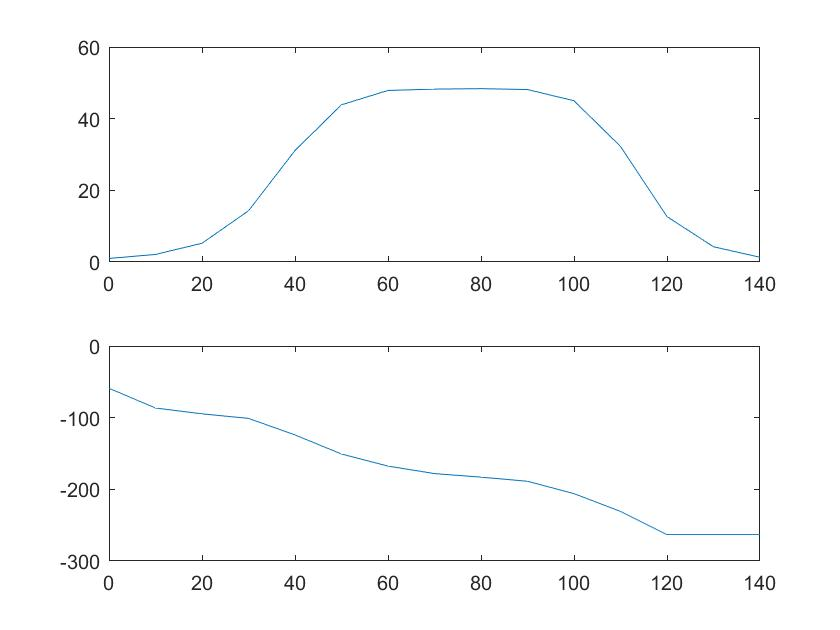
\includegraphics[width=\textwidth]{bode2exp.jpg}
\caption{$I_{CQ}=2\rm{mA}$时的辐频相频特性图}
\label{bode2}
\end{figure}
\section{传递函数的估计}
\section{传递函数形式的估计}
根据如图\ref{refin1}所示的折线化之后的bode图可以迅速得到两种情况下电路辐频特性的上升段和下降段的斜率为$\pm1$。表征单独考虑这一部分应当是一个一阶系统。同时,可以得到对于$I_{CQ}=1\rm{mA}$时的转折频率为46.93dB和106.9dB,
根据图\ref{bode1}提示的相频特性可以通过控制理论知识迅速得到这不是一个最小相位系统,因此先通过最小相位系统确定符合辐频特性的传递函数再根据相位进行进一步的调整

计算得到两个转折频率为222.075Hz和221.3kHz,同时辐频响应提示一个PD(超前环节)和一个PI(滞后环节)的综合,因此可以猜测系统的传递函数为

\begin{equation}
G'(s)=K\frac{T_1s+1}{4.5\times10^{-3}s+1}\times\frac{T_2s+1}{4.5\times10^{-6}s+1}, T_1>0,T_2>0
\end{equation}
\begin{figure}
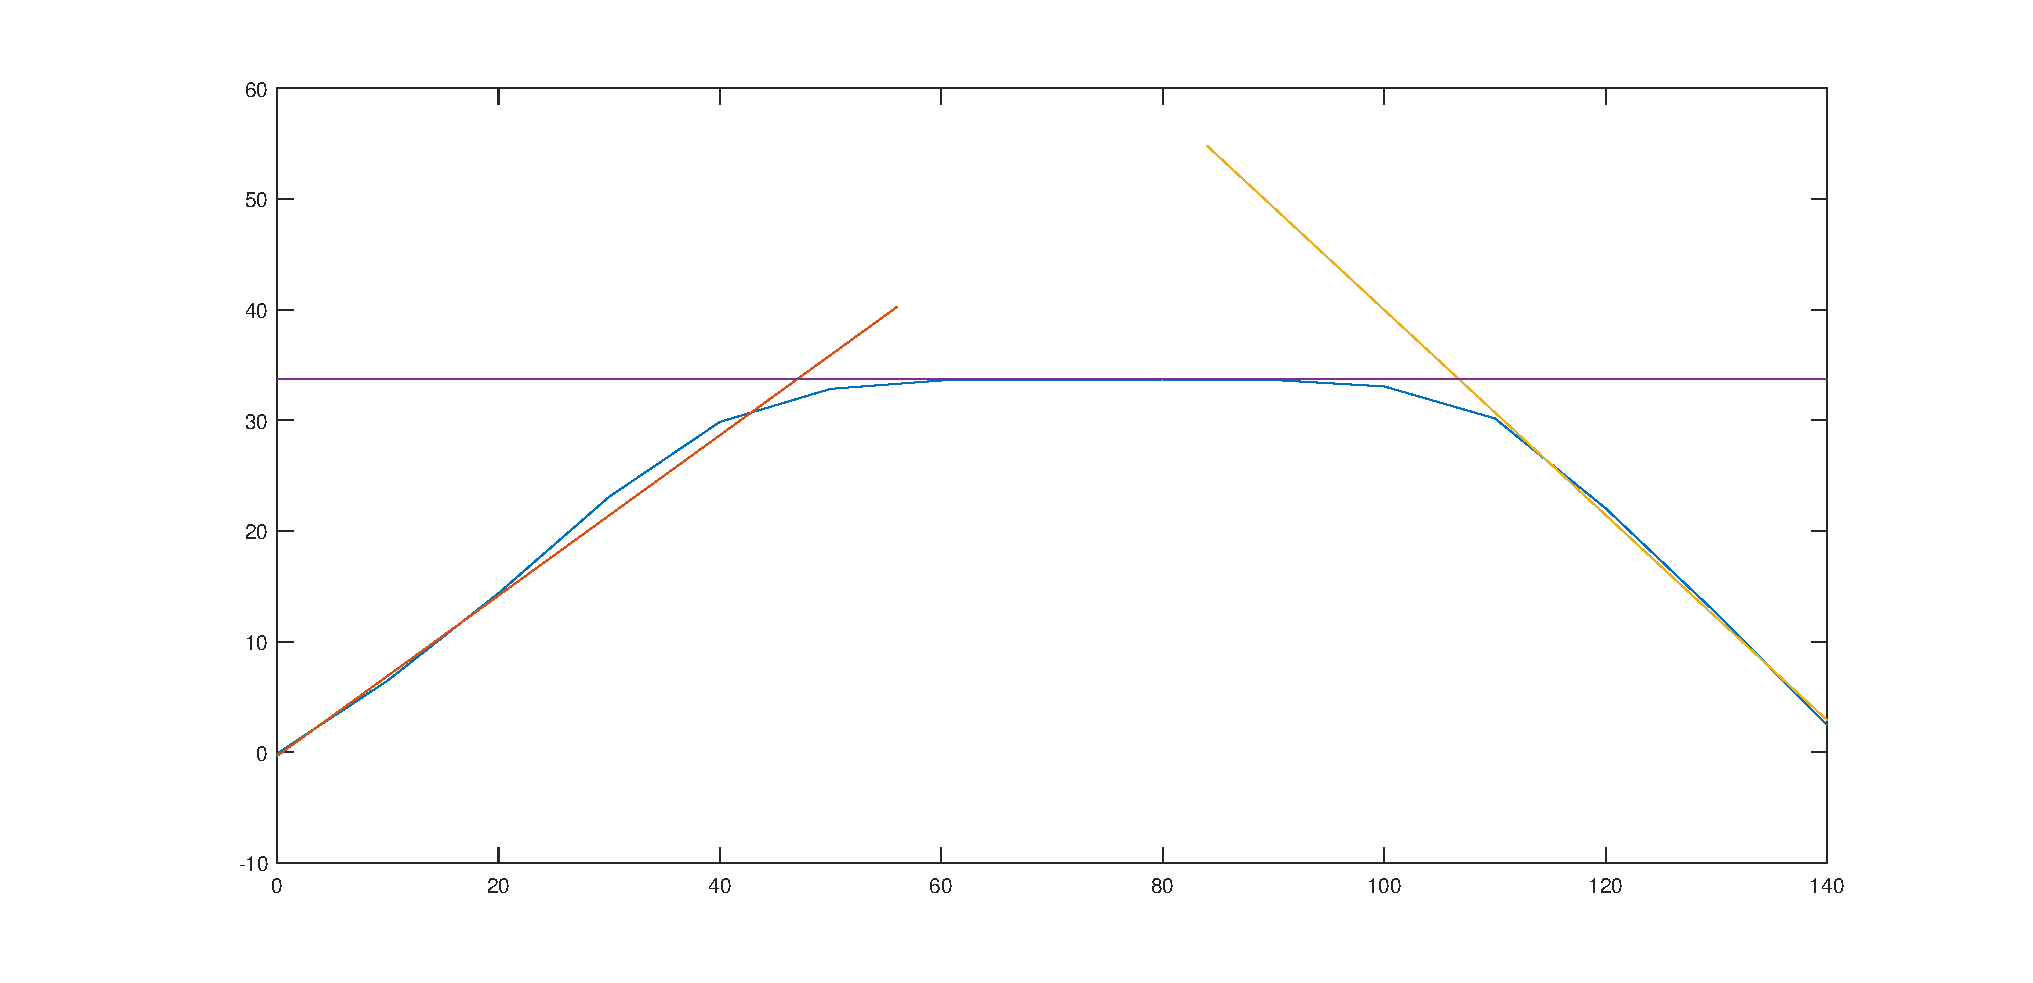
\includegraphics[width=\textwidth]{bode1.eps}
\caption{折线化之后的辐频响应}
\label{refin1}
\end{figure}
观察相频特性\ref{bode1}可得,系统相位不断滞后,又考虑到系统开环稳定,没有右半平面的极点,因此可以得到更正过的传递函数
\begin{equation}
G(s)=K\frac{-T_1s+1}{4.5\times10^{-3}s+1}\times\frac{T_2s+1}{4.5\times10^{-6}s+1}, T_1>0,T_2>0
\end{equation}
\section{时间参数的估计}
由于辐频特性中没有提示其他的拐点,因此我们希望通过相频特性寻找$T_1,T_2$的合理估计值

从控制理论我们可以知道,作为一个合理的近似,我们可以知道$G(s)$表达式中的左侧部分对高频特性影响较小,而右侧部分对低频特性影响较小,增益$k$不影响相频特性,因此我们分别对两个转折频率前后的频段进行研究

\begin{enumerate}
\item{低频部分}
经过研究发现,如果引入$T_1$,为了尽可能好的拟合低频部分的频率特性,发现在所研究的频段内均有$T_1\omega >> 1 $因此引入$T_1$变得意义不大,因此低频部分可以退化为$\frac{-s}{4.5\times10^{-3}s+1}$来简化传递函数
\item{高频部分}
经过研究发现,和低频部分相同的是,分子对相频特性的影响不大,因此,可以直接略去分子
\end{enumerate}
综上所述,系统的传递函数可以写成
\begin{equation}
G(s)=K\frac{-s}{4.5\times10^{-3}s+1}\times\frac{1}{4.5\times10^{-6}s+1}, T_1>0,T_2>0
\end{equation}

\subsection{增益K的估计}
根据中频段稳定特性对$K$进行估计可以得到K=0.23
\subsection{总结}
因此可以得到在研究频段特性为
\begin{equation}
G(s)=\frac{-0.23s}{(4.5\times10^{-3}s+1)(4.5\times10^{-6}s+1)}
\end{equation}
\end{document}